\documentclass[8pt]{beamer}
\usepackage{amsmath}
\usepackage{amssymb}
\usepackage[style=ieee]{biblatex}
\addbibresource{references.bib}
\usepackage{graphicx}
\usepackage{booktabs}
\usepackage{multirow}
\usepackage{lscape}
\usepackage{longtable}
\usepackage{hyperref}

\usetheme{PaloAlto}

\title{Detecting abnormalities on chest X-rays using deep neural networks}
\author{
  Swaroop Kumar M L\\
  Department of Studies in Computer Science\\
  University of Mysore
}
\date{\today}

\begin{document}
\maketitle

\section{Introduction}

\begin{frame}
  \frametitle{Abstract} Inspired by previous work, we develop algorithms that
  can detect abnormalities on the x-ray. The algorithm explains these detections
  by generating heatmaps pointing out areas of the image that most influenced
  it. \pause We establish baselines, benchmark against previous work and show
  that \pause
  \begin{itemize}
  \item{Transfer-learning from a large non-TB dataset dramatically improves TB
      detection}\pause
  \item{Models in the domain show inferior performance on external data from a
      different hospital system, but}\pause
  \item{Recent techniques such as mixup and progressive resizing improve
      performance and generalization.}\pause
  \end{itemize}
  We achieve performance competitive with previous work in detecting
  pneumonia-like and other abnormalities on the NIH chestX-ray14 dataset and
  \pause in detecting tuberculosis on the Shenzhen hospital dataset, and achieve
  state-of-the-art performance on the Montgomery county tuberculosis dataset.
  \pause We look for potential sources of bias and evaluate our baseline with
  respect to gender, age and view position.
\end{frame}

\begin{frame}
  \frametitle{Problem definition}

  \begin{columns}

    \column{.5\textwidth} When air in the alveoli is replaced with pus, blood
    and other fluids, referred to as consolidation and commonly caused by
    pneumonia, or when abscesses in the lung rupture forming cavities,
    indicating a tuberculosis infection, these are visible on the chest x-ray.\\
    \pause

    \column{.5\textwidth}
    \begin{figure}
      % \fbox{
      % \begin{minipage}{\textwidth}
      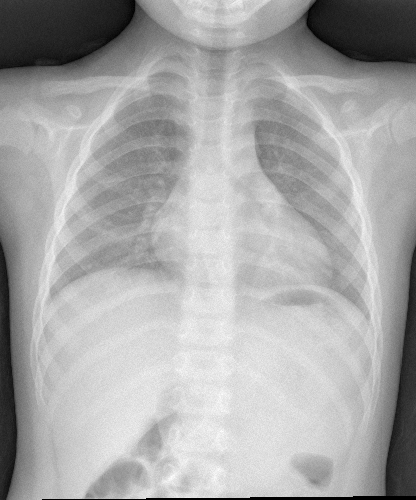
\includegraphics[width=0.3\textwidth]{images/normal1}\hspace{0.01\textwidth}%
      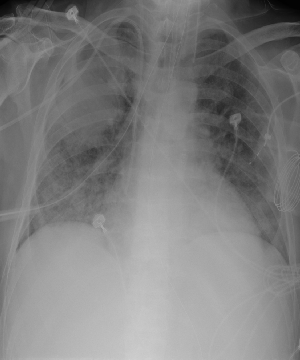
\includegraphics[width=0.3\textwidth]{images/consolidation_original}\hspace{0.01\textwidth}%
      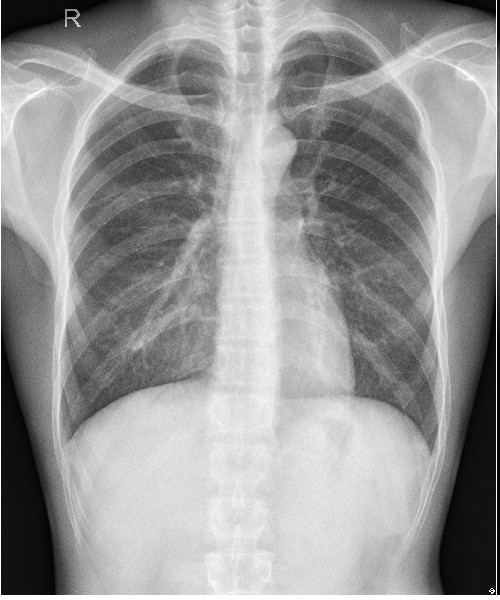
\includegraphics[width=0.3\textwidth]{images/TB_original}\\[0.01\textwidth]
      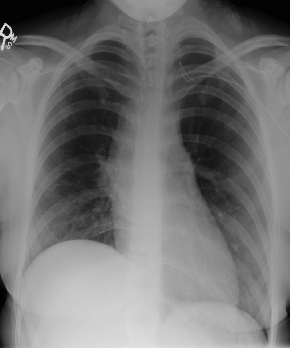
\includegraphics[width=0.3\textwidth]{images/normal2}\hspace{0.01\textwidth}%
      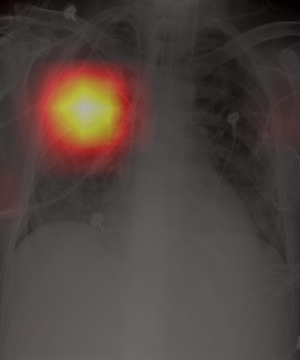
\includegraphics[width=0.3\textwidth]{images/consolidation_heatmap}\hspace{0.01\textwidth}%
      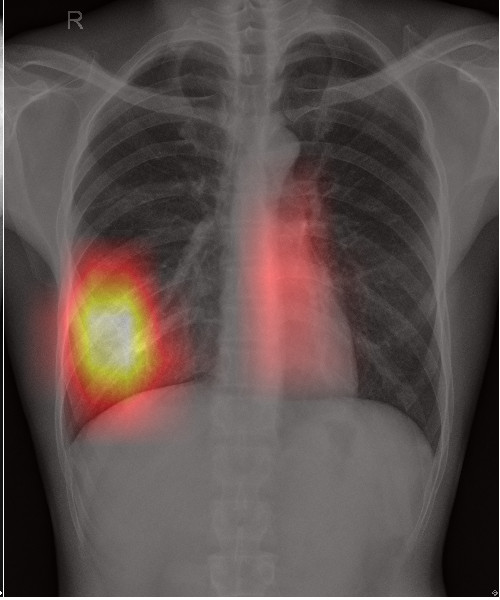
\includegraphics[width=0.3\textwidth]{images/TB_heatmap}
      \caption{From left to right: The first column shows two \emph{Normal}
        images. Columns 2 and 3 show images with \emph{Pneumonia} and
        \emph{Tuberculosis} respectively, the first row showing the original
        images and the second showing the same overlaid with heatmaps localizing
        the abnormalities, which we call \emph{examples}}
      % \end{minipage}
      % }
      \label{basic_examples}
    \end{figure}

  \end{columns}
\end{frame}

  \begin{frame}
    An algorithm that can automatically detect these abnormalities can be useful
    in numerous ways.\\ \pause \vspace{\baselineskip}
    \begin{enumerate}
    \item{For active case finding in high-risk populations, for example, with
        mobile x-ray vans\cite{modi_suresh_2019}}\pause
    \item{As an initial screening test before or along with other tests such as
        a sputum examination}\pause
    \item{To aid a radiologist in her workflow by sorting her queue based on
        severity, suggesting areas to consider in an image, providing a second
        opinion, etc.}\pause
    \end{enumerate}

    \vspace{\baselineskip}
    
    Our work focuses on the core algorithm. We divide the problem into, and
    explore, four sub-problems.


  \end{frame}

  \begin{frame}

    \frametitle{Classification} For our primary dataset, a large collection of
    chest x-rays annotated with multiple abnormalities including pneumonia
    \cite{Wang2017a}, we formulate the problem as a multi-class multi-label
    classification problem.\pause \\
    \vspace{\baselineskip} The task is to learn a function $f:X \rightarrow 2^L$
    \\ \pause \vspace{\baselineskip}
    For the Shenzhen hospital tuberculosis dataset\cite{jaeger2014two}, we formulate the problem as a binary classification problem. \\
    \pause \vspace{\baselineskip} The task is to learn a function $f:X
    \rightarrow \{\,0, 1 \,\}$

  \end{frame}

  \begin{frame}

    \frametitle{Explainability} Deep neural networks have outperformed previous
    methods in several domains. However, they remain black-boxes with millions
    of parameters, leading to a lack of trust and limiting their use in routine
    clinical practice. \\ \pause \vspace{\baselineskip} Several methods have
    been proposed to make these models more interpretable, broadly falling into
    two categories:
    \begin{enumerate}
    \item{Methods that create a proxy model} \pause
    \item{Methods that generate a saliency map} \pause
    \end{enumerate}
    \vspace{\baselineskip} Given an input $x = \{\, x_{1}, x_{2}, x_{3} \dots
    x_{n} \,\} \in X$, and a set of class labels $L = \{\,l_1 ,l_2 ,l_3 \dots
    l_c\,\}$, the task is to compute the attribution
    \begin{equation}
      A_j = \{\,a_{j1}, a_{j2}, a_{j3} \dots a_{jn}\,\} \in \mathbb{R} ^n
    \end{equation}
    for each class $l_j \in L$ where $a_{ji} \in A_j$ is a measure of the
    relevance of
    the $i^{th}$ feature to the model's inference regarding the $j^{th}$ class.\\


  \end{frame}

  \begin{frame}
    \frametitle{Generalizability} A test set is considered representative of
    data that will be encountered in the external world and is used exclusively
    to evaluate a model. However, true generalization to new datasets may be
    lower than expected. \\ \pause

    \vspace{\baselineskip}

    Two datasets may have different distributions. In the context of biomedical
    imaging, datasets may be collected from different hospital systems and
    machines. \\ \pause

    \vspace{\baselineskip}

    The dataset used to train a model may have confounding variables that do not
    exist in other datasets. For example, in \cite{zech2018variable}, Zech et
    al. show that CNNs were able to directly detect the hospital system and
    department within a hospital system from a chest radiograph where saliency
    maps showed high activation in image corners.
    
  \end{frame}

  \begin{frame}
\frametitle{Weighted average of saliency maps}
\begin{figure}[H]
  % \fbox{
  % \begin{minipage}{\textwidth}
  \centering \emph{a}
  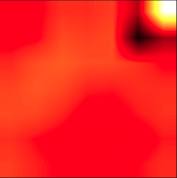
\includegraphics[width=0.28\textwidth]{images/heatmap_224_noda}\hspace{0.01\textwidth}%
  \emph{b}
  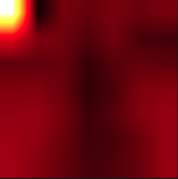
\includegraphics[width=0.28\textwidth]{images/heatmap_224_da}\hspace{0.01\textwidth}%
  \emph{c} 
\includegraphics[width=0.28\textwidth]{images/heatmap_224_cropped}\\[0.01\textwidth]
  \hspace{0.15\textwidth} \emph{e}
  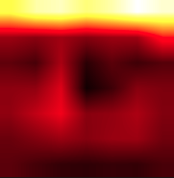
\includegraphics[width=0.28\textwidth]{images/heatmap_224_no_in}\hspace{0.01\textwidth}%
  \emph{d} 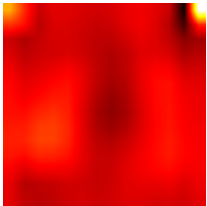
\includegraphics[width=0.28\textwidth]{images/heatmap_224_guangzhou}\hspace{0.15\textwidth}\\[0.01\textwidth]
  \caption{Average saliency maps for \emph{pneumonia}. Clockwise from the
    top-left: a) Baseline, b) Baseline with more data augmentation, c) Trained
    with margins cropped, d) Trained on NIH CXR-14, tested on Guangzhou and e)
    Trained without pre-training on ImageNet }
  % \end{minipage}
  % }
  \label{avg_saliency_maps}
\end{figure}
  \end{frame}

  \begin{frame}
    \frametitle{Fairness}

    Algorithms may inadvertently learn and leverage biases in the datasets,
    discriminate based on race, gender, etc. and amplify existing social
    inequities. \\ \pause

    \vspace{\baselineskip}

    In \cite{buolamwini2018gender}, Buolamwini et al. show that facial
    recognition datasets are overwhelmingly composed of light-skinned
    individuals and that commercial gender classification systems performed
    worse for dark-skinned people and females, with a difference in accuracy of
    more than 30\% between light-skinned males and dark-skinned females. \\
    \pause

    \vspace{\baselineskip}

    A simple measure against bias could be to hide variables like gender and
    race from a model, but complex machine learning models learn to use other
    correlated variables as proxy for hidden ones (for example, zipcode as
    correlated with race and the word `women' in an institution's name as
    correlated with the gender of its students\cite{dastin_2018}).

  \end{frame}

  \begin{frame}

    We measure the potential for discrimination by
    % \begin{enumerate}
    % \item{Measuring the correlation of various abnormalities with gender and
    %   age
    %   group}
    % \item{
    training models with architectures similar to the abnormality detection
    model, to identify gender and age group from images alone.
    % }
    % \end{enumerate}
    We then test our baseline model's performance across genders and age groups.
  
  \end{frame}

  \section{Data}

  \begin{frame}
\frametitle{Data}
    We use the NIH ChestX-ray14 dataset\cite{Wang2017} and the Shenzhen hospital
    tuberculosis dataset\cite{jaeger2014two} to train models to detect pneumonia
    and other abnormalitites, and tuberculosis respectively. \\ \pause

    \vspace{\baselineskip}
    
    We then use two external datasets, the Guangzhou medical center pediatric
    pneumonia dataset\cite{kermany2018identifying} and the Montgomery county
    tuberculosis dataset\cite{jaeger2014two} as \emph{external} datasets to test
    the ability of these models to generalize to other hospital systems.

  \end{frame}

  \begin{frame}
    \begin{table}[]
      \centering
      \begin{tabular}{@{}llll@{}}
        \toprule
        \textbf{}                              & \textbf{Training} & \textbf{Testing} & \textbf{\begin{tabular}[c]{@{}l@{}}Different\\ Hospital system?\end{tabular}} \\ \midrule
        \multirow{3}{*}{\textbf{Pneumonia}}    & NIH CXR-14        & NIH CXR-14       & No                                                                            \\ \cmidrule(l){2-4} 
                                               & NIH CXR-14        & Guangzhou   & Yes                                                                           \\ \cmidrule(l){2-4} 
                                               & Guangzhou    & Guangzhou   & No                                                                            \\ \midrule
        \multirow{3}{*}{\textbf{Tuberculosis}} & Shenzhen          & Shenzhen         & No                                                                            \\ \cmidrule(l){2-4} 
                                               & Shenzhen          & Montgomery       & Yes                                                                           \\ \cmidrule(l){2-4} 
                                               & Montgomery        & Montgomery       & No                                                                            \\ \bottomrule
      \end{tabular}
      \caption{Datasets used for training and testing}
      \label{tab:test-combos}
    \end{table}
  \end{frame}

  \begin{frame}
    \frametitle{NIH CXR-14} The NIH chestX-ray14 dataset consists of 112,120
    chest x-ray images of 30,805 unique patients which was collected using the
    PAC system of the National Institutes of Health. Each image was labeled with
    up-to 14 abnormalities
    algorithmically using the associated radiology report in natural language. \\
    \pause

    \vspace{\baselineskip}

    About half or 60,361 of these are labeled as \emph{No finding} and the rest
    are labeled with one of more of the 14 abnormalities. Some abnormalities are
    more common than others, the most common being \emph{Infiltration}, which is
    present in 19,894 images, and the least common being \emph{Hernia}, which is
    present in only 227 images.\\ \pause

    \vspace{\baselineskip}

    We split the dataset into train, validation and test sets roughly in the
    ratio 70:10:20. We make sure that there is no patient overlap, that is, all
    images of a patient are in the same subset since patient overlap may lead to
    overfitting.


  \end{frame}

\begin{frame}
  \tiny{
    \begin{table}[]
      \centering
      \begin{tabular}{@{}lllll@{}}
        \toprule
        \textbf{Abnormality} & \multicolumn{4}{l}{\textbf{Number of images}}        \\ \midrule
                             & Train     & Validation & Test      & Total           \\ \midrule
        Atelectasis          & 7996      & 1119       & 2420      & 11559           \\ \midrule
        Cardiomegaly         & 1950      & 240        & 582       & 2776            \\ \midrule
        Effusion             & 9261      & 1292       & 2754      & 13317           \\ \midrule
        Infiltration         & 13914     & 2018       & 3938      & 19894           \\ \midrule
        Mass                 & 3988      & 625        & 1133      & 5782            \\ \midrule
        Nodule               & 4375      & 613        & 1335      & 6331            \\ \midrule
        Pneumonia            & 978       & 133        & 242       & 1431            \\ \midrule
        Pneumothorax         & 3705      & 504        & 1089      & 5302            \\ \midrule
        Consolidation        & 3263      & 447        & 957       & 4667            \\ \midrule
        Edema                & 1690      & 200        & 413       & 2303            \\ \midrule
        Emphysema            & 1799      & 208        & 509       & 2516            \\ \midrule
        Fibrosis             & 1158      & 166        & 362       & 1686            \\ \midrule
        Pleural Thickening   & 2279      & 372        & 734       & 3385            \\ \midrule
        Hernia               & 144       & 41         & 42        & 227             \\ \midrule
        No Finding           & 42405     & 6079       & 11928     & 60361           \\ \midrule
        \textbf{Total}       & \textbf{78468} & \textbf{11219}  & \textbf{22433} & \textbf{112120} \\ \bottomrule
      \end{tabular}
      \caption{For the NIH CXR-14 dataset, the number of images in the train,
        validation and test sets per abnormality}
      \label{tab:nih_split}
    \end{table}
  }
\end{frame}

\begin{frame}
  \frametitle{Challenges and issues}
  \begin{enumerate}
  \item{\textbf{Noisy labels}\\
      Labels were extracted using NLP from radiology reports in natural language
      text. This may lead to label noise. \cite{Wang2017} show that these labels
      are about 90\% accurate. Although deep neural networks have been shown to
      be robust to label noise in general\cite{rolnick2017deep}, structured
      noise can be especially detrimental to performance.} \pause
  \item{\textbf{Labeling schema}\\
      Some of these abnormalities are sub-types of others, but labels are
      provided as a non-hierarchical list. For example, \emph{Pneumonia} on the
      x-ray is a form of \emph{Consolidation} } \pause
  \item{\textbf{Class imbalance}\\
      The majority of images do not contain abnormalities, and some
      abnormalities are common while others are rare. For example,
      \emph{Infiltration} appears in 17\% of the images while \emph{Hernia}
      appears in only 0.2\% of the images.}
  \end{enumerate}
\end{frame}

\begin{frame}
  \frametitle{Guangzhou} The Guangzhou pediatric pneumonia dataset consists of
  8,497 chest x-ray images of children under the age of 5 years collected from
  the Guangzhou Women and Children’s Medical Center, Guangzhou. Each image has
  been labeled as either \emph{Normal} (4232 images) or \emph{Pneumonia} (4265
  images). Images labeled as \emph{Pneumonia} have been further tagged as
  \emph{Bacterial} (2772 images) or \emph{Viral} (1493 images) based on the
  cause of pneumonia.\\ \pause

  \vspace{\baselineskip}

  We use the standard test set and split the rest of the dataset into train and
  validation sets in the ratio 80:20. However, when used as an external dataset,
  we use the entire dataset.
\end{frame}

\begin{frame}
  \begin{table}[]
    \centering
    \begin{tabular}{@{}lllll@{}}
      \toprule
      \textbf{Label}      & \multicolumn{4}{l}{\textbf{Number of images}}  \\ \midrule
                          & Train     & Validation & Test      & Total     \\ \midrule
      Normal              & 3199      & 799        & 234       & 4232           \\ \midrule
      Viral pneumonia     & 1076      & 269        & 148       & 1493          \\ \midrule
      Bacterial pneumonia & 2024      & 506        & 242       & 2772          \\ \midrule
      \textbf{Total}      & \textbf{6299} & \textbf{1574}  & \textbf{624} & \textbf{8497} \\ \bottomrule
    \end{tabular}
    \caption{For the Guangzhou pediatric pneumonia dataset, the number of images
      in the train, validation and test sets per label}
    \label{tab:guangzhou_split}
  \end{table}


\end{frame}

\begin{frame}
  \frametitle{Shenzhen} The Shenzhen tuberculosis dataset consists of 615 chest
  x-ray images collected from the Shenzhen No.3 Hospital in Shenzhen, Guangdong
  providence, China. Each of the images is labeled as either \emph{Normal} or
  \emph{Tuberculosis}. 340 of these are normal and 275 show manifestations of
  tuberculosis.\\ \pause

  \vspace{\baselineskip}

  Considering the small size of the dataset, we create 9 folds of the dataset
  and report average and standard deviation of metrics. Each fold contains all
  the images split into train, validation and test sets in the ratio 70:10:20.


\end{frame}

\begin{frame}

  \frametitle{Montgomery}

  The Montgomery county tuberculosis dataset consists of 138 chest x-ray images
  collected from the tuberculosis control program of the Department of Health
  and Human Services of Montgomery County, MD, USA. Each of the images is
  labeled as either \emph{Normal} or \emph{Tuberculosis}. 80 of these are normal
  and 58 show manifestations of tuberculosis. The dataset also contains manually
  segmented lung masks for each image.\\ \pause

  \vspace{\baselineskip}

  Similar to the Shenzhen dataset, we create 9 folds and report average and
  standard deviation of metrics. Each fold contains all the images split into
  train, validation and test sets in the ratio 70:10:20. However, when used as
  an external dataset, we ignore these folds and test on the entire dataset.

\end{frame}

\section{Baselines}

\begin{frame}
  \frametitle{Model architecture}
  
  We replace the final fully connected layer of 121-layer dense convolutional
  neural network with one that has either 14 outputs (for the NIH CXR-14
  dataset) or 2 outputs (for all other datasets) after which we apply a sigmoid
  non-linearity. \\ \pause

  \vspace{\baselineskip}

  The fully convolutional backbone of the network results in $k$ $w$ x $h$
  feature maps and is followed by a global-average-pooling layer where the $k$
  feature maps are averaged along the width and height to form a $k$ dimensional
  vector.
\end{frame}


\begin{frame}
  \begin{figure}
    \centering 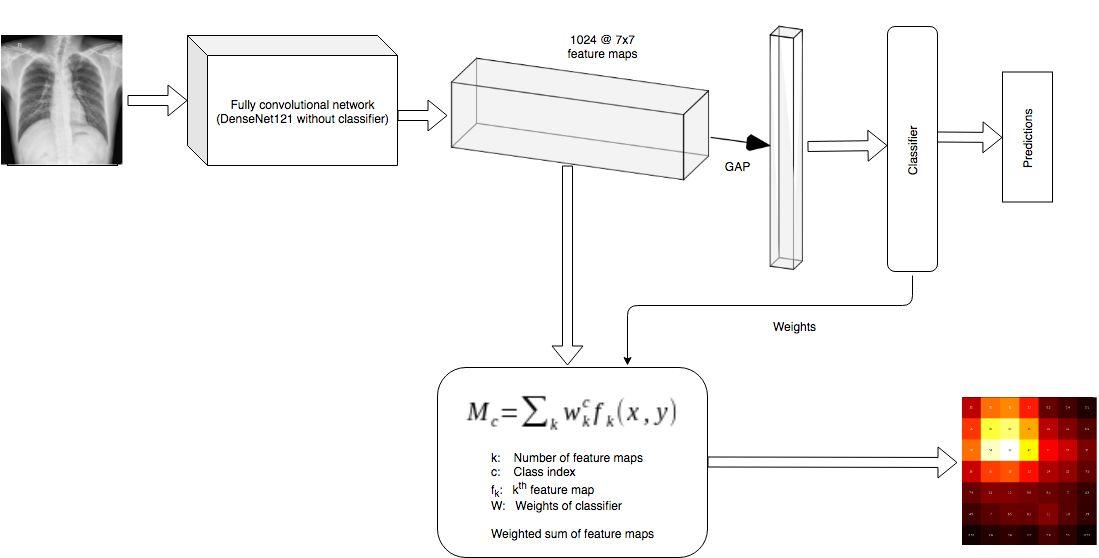
\includegraphics[width=\textwidth]{images/arch}
    \caption{Basic architecture of the model}
    \label{architecture}
  \end{figure}
\end{frame}

  \begin{frame}
    \frametitle{Inference}

    At the multi-class multi-label classification task (for the NIH CXR-14
    dataset), we merge the train and validation sets after training and use it
    to compute optimal thresholds for each abnormality by optimizing for the
    class-specific F1-score.\\ \pause

    \vspace{\baselineskip}

    Although it is possible to compute optimal thresholds for the classification
    task since we have ground truth labels, it is not possible to do so for the
    localization task since we only have weak labels and not precise location.\\
    \pause

    \vspace{\baselineskip}

    At binary classification tasks, since the network has two output nodes, we
    do not compute thresholds but simply consider as the proper output the class
    whose corresponding output node has higher activation.
  \end{frame}

    \begin{frame}
      \frametitle{Computing saliency maps} To compute explanations, we save the
      feature maps resulting from the final convolutional layer during a forward
      pass and perform a weighted sum of these feature maps using the weights of
      the final fully-connected layer between
      each of the feature maps and the desired output node, as follows.\\ \pause

      \vspace{\baselineskip}

      If $f_i$ is the $i^{th}$ feature map and $w^j _i$ is the weight between
      the $i^{th}$ input node and the $j^{th}$ output node in the
      fully-connected layer, the saliency map for the $j^{th}$ class $M_j$ is
      \begin{equation}
        M_j = \sum _i \, w^j _i \, f_i
      \end{equation}
      $M_j$ is a $w$ x $h$ saliency map which we interpolate to the size of the
      input image and visualize as a heatmap
    \end{frame}

      \begin{frame}
        We use a region-growing algorithm to determine bounding boxes given a
        saliency map. Specifically, we first threshold the saliency map and
        using the maximum element as a seed point, grow a region around it,
        including all non-zero neighbours, and repeat the same until all
        non-zero elements are included in a region, each time choosing as seed
        the maximum element not included a region. For each region, we determine
        a bounding box as the smallest rectangle which encloses the entire
        region.
      \end{frame}

      \begin{frame}
        \begin{figure}
          \centering
          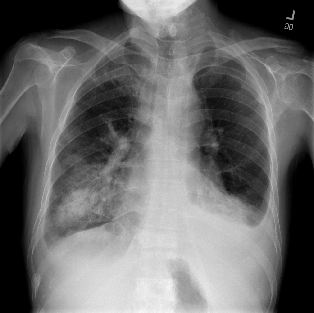
\includegraphics[height=0.4\textheight]{images/pneumonia_orig}\hspace{0.01\textwidth}%
          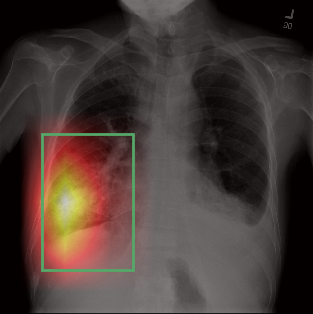
\includegraphics[height=0.4\textheight]{images/pneumonia_hm_bbox}\\[0.01\textwidth]
          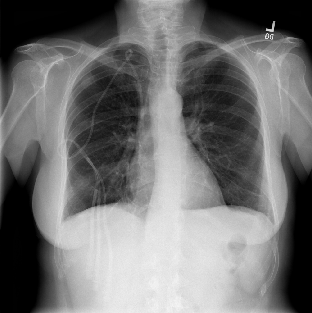
\includegraphics[height=0.4\textheight]{images/atelectasis_orig}\hspace{0.01\textwidth}%
          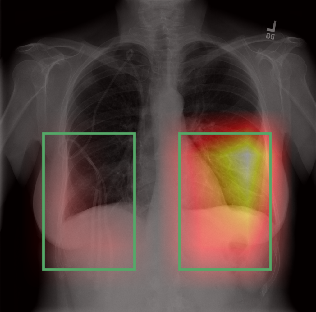
\includegraphics[height=0.4\textheight]{images/atelectasis_hm_bbox}\\[0.01\textwidth]
          \caption{Examples of saliency maps with corresponding bounding boxes
            drawn. The first column shows original x-ray images and the second
            row shows saliency map and bounding boxes overlaid on the image. Row
            1: Pneumonia. Row 2: Atelectasis.}
          \label{cam_bbox_examples}
        \end{figure}


      \end{frame}

      \begin{frame}

        \frametitle{Evaluation metrics}

        We primarily use the area under the reciever-operator-characteristic
        curve (AUROC) to measure the performance of a model. AUROC is not
        affected by the class distribution, does not need thresholds to be set,
        and is commonly used in the literature. Apart from AUROC and accuracy,
        we also use \\ \pause

        \vspace{\baselineskip}

        \begin{enumerate}
        \item{\textbf{Specificity}\\
            \begin{equation}
              Specificity = \frac{|TN|}{|TN| + |FP|}
            \end{equation}
          }
        \item{\textbf{Sensitivity}\\
            \begin{equation}
              Sensitivity = \frac{|TP|}{|TP| + |FN|}
            \end{equation}
          }
        \end{enumerate}

      \end{frame}


      \begin{frame}
        \frametitle{Baseline results}
        \begin{table}[]
          \centering
          \begin{tabular}{@{}ll@{}}
            \toprule
            \textbf{Abnormality} & \textbf{AUROC} \\ \midrule
            Atelectasis          & 0.823          \\ \midrule
            Cardiomegaly         & 0.905          \\ \midrule
            Effusion             & 0.879          \\ \midrule
            Infiltration         & 0.712 \\ \midrule
            Mass                 & 0.839          \\ \midrule
            Nodule               & 0.778 \\ \midrule
            Pneumonia            & 0.760          \\ \midrule
            Pneumothorax         & 0.869          \\ \midrule
            Consolidation        & 0.806 \\ \midrule
            Edema                & 0.891          \\ \midrule
            Emphysema            & 0.923          \\ \midrule
            Fibrosis             & 0.831 \\ \midrule
            Pleural\_Thickening  & 0.785          \\ \midrule
            Hernia               & 0.929          \\ \midrule
            \textbf{Average}     & \textbf{0.838}          \\ \bottomrule
          \end{tabular}
          \caption{Baseline results on the NIH CXR-14 dataset}
          \label{tab:baseline_nih}
        \end{table}

      \end{frame}
      \begin{frame}

\begin{table}[]
  \centering
  \begin{tabular}{@{}lllll@{}}
    \toprule
    & \textbf{AUROC} & \textbf{Accuracy} & \textbf{Specificity} & \textbf{Sensitivity} \\ \midrule
    Mean               & 0.956          & 0.902             & 0.902                & 0.899                \\ \midrule
    Standard deviation & 0.009          & 0.019             & 0.050                & 0.045                \\ \bottomrule
  \end{tabular}
  \caption{Baseline results on the Shenzhen hospital tuberculosis dataset}
  \label{tab:baseline_shenzhen}
\end{table}

\end{frame}

\section{Experiments}
        \begin{frame}
          \frametitle{Experiments}
          \begin{enumerate}
          \item{Data augmentation} \pause
          \item{Test-time augmentation}\pause
          \item{Mixup}\pause
          \item{Transfer-learning from ImageNet}\pause
          \item{Transfer-learning from NIH CXR-14}\pause
          \item{Over-diagnosis of TB}\pause
          \item{Progressive resizing}\pause
          \item{Ensembling predictions}\pause
          \item{Ensembling saliency maps}\pause
          \item{Cropping of image margins}\pause
          \item{Fairness}\pause
          \item{Generalization}\pause
             
          \end{enumerate}

        \end{frame}

        \section{Results}
        
          \begin{frame}
            \frametitle{Comparison to previous work on NIH CXR-14}
            \begin{table}[]
              \centering
              \begin{tabular}{ll}
                \hline
                \textbf{Authors}            & \textbf{Average AUROC} \\ \hline
                Wang et al. (2017)          & 0.738                  \\ \hline
                Y. Shen et al.              & 0.775                  \\ \hline
                H. Wang et al. (ChestNet)   & 0.781                  \\ \hline
                P. Kumar et al.             & 0.792                  \\ \hline
                Yao et al. (2017)           & 0.803                  \\ \hline
                Y. Tang et al.              & 0.805                  \\ \hline
                S. Guendel et al.           & 0.807                  \\ \hline
                Yan et al.                  & 0.83                   \\ \hline
                X. Xu et al. (DeepCXray)    & 0.832                  \\ \hline
                Rajpurkar et al. (CheXNet)  & 0.841                  \\ \hline
                B. Zhou et al.              & 0.842                  \\ \hline
                Rajpurkar et al. (ChexNext) & 0.849                  \\ \hline
                \textbf{Our model}          & \textbf{0.856}         \\ \hline
                Q. Guan et al.              & 0.871                  \\ \hline
              \end{tabular}
              \caption{Comparison to previous work on the NIH CXR-14 dataset}
              \label{tab:nih_previous}
            \end{table}

          \end{frame}

\begin{frame}
  \frametitle{Comparison to human radiologists} Rajpurkar et al. in
  \cite{Rajpurkar2018a} measured human performance in terms of AUROC for each
  disease, using the majority vote of 3 independent board-certified
  cardiothoracic specialist radiologists (average experience 15 years) as ground
  truth, and measure the the performance of 6 BC radiologists from 3 academic
  institutions (average experience 12 years) and 3 senior radiology residents by
  fitting a curve to these 9 radiologists' operating points and calculating the
  area under it.
\end{frame}

\begin{frame}
  \begin{table}[]
    \centering
    \begin{tabular}{lllll}
      \hline
      \textbf{Abnormality} & \multicolumn{4}{l}{\textbf{AUROC}}             \\ \hline
                           & Baseline & Ensemble & Radiologist & Difference (\%) \\ \hline
      Atelectasis          & 0.823    & 0.839    & 0.808       & -3.06      \\ \hline
      Cardiomegaly         & 0.899    & 0.916    & 0.888       & -2.79      \\ \hline
      Effusion             & 0.881    & 0.89     & 0.9         & 0.96       \\ \hline
      Infiltration         & 0.705    & 0.72     & 0.734       & 1.39       \\ \hline
      Mass                 & 0.857    & 0.868    & 0.886       & 1.76       \\ \hline
      Nodule               & 0.779    & 0.817    & 0.899       & 8.17       \\ \hline
      Pneumonia            & 0.767    & 0.765    & 0.823       & 5.83       \\ \hline
      Pneumothorax         & 0.881    & 0.895    & 0.94        & 4.46       \\ \hline
      Consolidation        & 0.822    & 0.819    & 0.841       & 2.22       \\ \hline
      Edema                & 0.911    & 0.902    & 0.91        & 0.83       \\ \hline
      Emphysema            & 0.913    & 0.944    & 0.911       & -3.33      \\ \hline
      Fibrosis             & 0.824    & 0.854    & 0.897       & 4.31       \\ \hline
      Pleural\_Thickening  & 0.81     & 0.805    & 0.779       & -2.59      \\ \hline
      Hernia               & 0.906    & 0.944    & 0.985       & 4.1        \\ \hline
      \textbf{Average}              & \textbf{0.841}    & \textbf{0.856}    & \textbf{0.8715}      & \textbf{1.59}       \\ \hline
    \end{tabular}
    \caption{Comparison to human radiologists on the NIH CXR-14 dataset}
    \label{tab:nih_comparision}
  \end{table}


\end{frame}

\begin{frame}
  \frametitle{Caveats with comparison to human radiologists}

  Overestimating model performance
  \begin{enumerate}
  \item{Noisy labels. Model may be overfitting to noise.}
  \item{Model may be overfitting to certain hospitals and machines.}
  \item{Model may be exploiting spurious correlations such as using presence of
      chest-drains to infer Pneumothorax.}
  \end{enumerate}
  \pause

  \vspace{\baselineskip}

  Underestimating human performance
  \begin{enumerate}
  \item{Unconventional labelling schema. Radiologists usually do not diagnose
      many of these abnormalities from x-rays. They have access to other
      clinical data}
  \item{Radiologists work with higher resolution images with more grey-levels
      than the dataset provides}
  \end{enumerate}
\end{frame}
  \begin{frame}
    \frametitle{Comparison to previous work on Shenzhen}
    \begin{table}[]
      \centering
      \begin{tabular}{lll}
        \hline
        \textbf{Authors}                    & \textbf{AUROC} &\textbf{Accuracy}\\ \hline
        Jaeger et al                        & 0.9            & 0.841\\ \hline
        Hwang et al                         & 0.93           & 0.837\\ \hline
        Lopez and Valiati                   & 0.926          & 0.846\\ \hline
        MT Islam et al                      & 0.94           & 0.9\\ \hline
        Haloi et al                         & 0.949          & \\ \hline
        Liu et al (ResNet-152)              & 0.967          & 0.923\\ \hline
        Liu et al (Inception-ResNet-v2)     & 0.983          & 0.917\\ \hline
        Vajda et al                         & 0.99           & 0.957\\ \hline
        \textbf{Our baseline}               & \textbf{0.956} & \textbf{0.902}        \\ \hline
        \textbf{\begin{tabular}[c]{@{}l@{}}Our best model\\ Pretrained on NIH CXR-14\\ with mixup $\alpha = 0.4$\end{tabular}} & \textbf{0.985}          & \textbf{0.949}\\ \hline
      \end{tabular}
      \caption{Comparison to previous work on the Shenzhen tuberculosis dataset}
      \label{tab:shenzhen_previous}
    \end{table}

  \end{frame}

  \begin{frame}
\frametitle{Comparison to previous work on Montgomery} 
\begin{table}[]
  \centering
  \begin{tabular}{lll}
    \hline
    \textbf{Authors}                   & \textbf{AUROC}  & \textbf{Accuracy}\\ \hline
    Jaeger et al                       & 0.869           & 0.783 \\ \hline
    Lopez and Valiati                  & 0.926           & 0.826 \\ \hline
    Liu et al (Inception-ResNet-v2)    & 0.957           & 0.844 \\ \hline
    Liu et al (ResNet-152)             & 0.951           & 0.890 \\ \hline
    Vajda et al                        & 0.870           & 0.783 \\ \hline
    \textbf{Our baseline}              & \textbf{0.871}  & \textbf{0.755}\\ \hline
    \textbf{\begin{tabular}[c]{@{}l@{}}Our best model\\ Pre-trained on NIH CXR-14\\ (480 x 480)\end{tabular}} & \textbf{0.957} & \textbf{0.89}\\ \hline
  \end{tabular}
  \caption{Comparison to previous work on the Montgomery tuberculosis dataset}
  \label{tab:montgomery_previous}
\end{table}


  
\end{frame}

\section{Examples}

\begin{frame}
\frametitle{Examples}
  \begin{figure}[H]
  % \fbox{
  % \begin{minipage}{\textwidth}
  \centering
  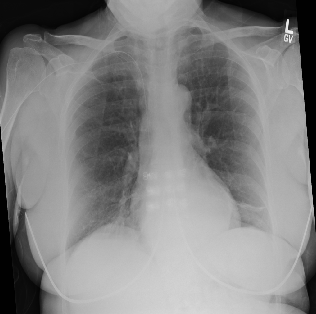
\includegraphics[width=0.3\textwidth]{images/preds/atelectasis}\hspace{0.01\textwidth}%
  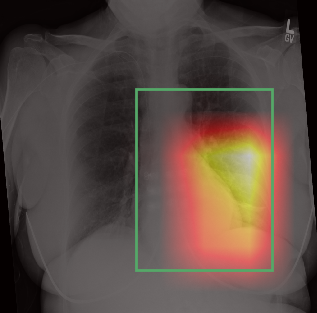
\includegraphics[width=0.3\textwidth]{images/preds/atelectasis_cam}\hspace{0.01\textwidth}%
  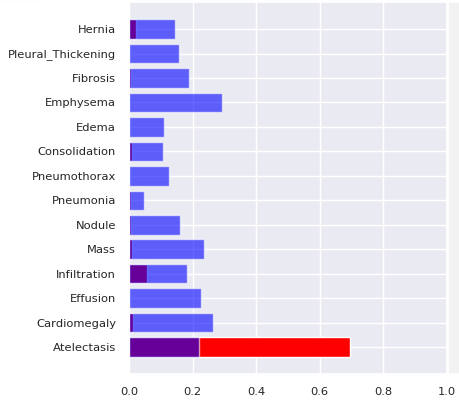
\includegraphics[width=0.3\textwidth]{images/preds/atelectasis_probs}\\[0.01\textwidth]
  \caption{Original image, image overlaid with saliency map and bounding boxes
    for \emph{Atelectasis}, and predicted probabilities for an x-ray image.}
  % \end{minipage}
  % }
  \label{examples_1}
\end{figure}\end{frame}

\begin{frame}
\begin{figure}[H]
  % \fbox{
  % \begin{minipage}{\textwidth}
  \centering
  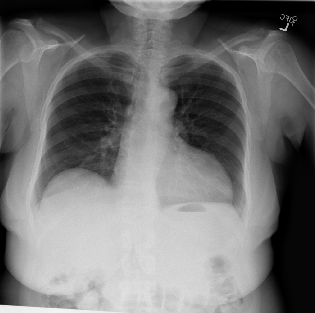
\includegraphics[width=0.3\textwidth]{images/preds/cardiomegaly}\hspace{0.01\textwidth}%
  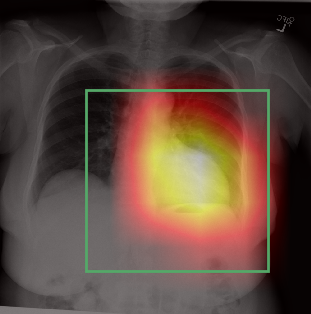
\includegraphics[width=0.3\textwidth]{images/preds/cardiomegaly_cam}\hspace{0.01\textwidth}%
  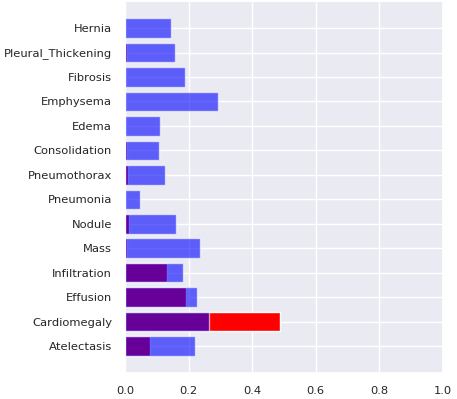
\includegraphics[width=0.3\textwidth]{images/preds/cardiomegaly_probs}\\[0.01\textwidth]
  \caption{Original image, image overlaid with saliency map and bounding boxes
    for \emph{Cardiomegaly}, and predicted probabilities for an x-ray image.}
  % \end{minipage}
  % }
  \label{examples_2}
\end{figure}
\end{frame}

\begin{frame}
\begin{figure}[H]
  % \fbox{
  % \begin{minipage}{\textwidth}
  \centering
  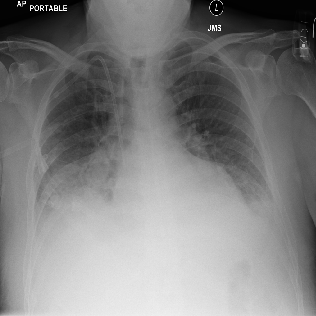
\includegraphics[width=0.3\textwidth]{images/preds/effusion}\hspace{0.01\textwidth}%
  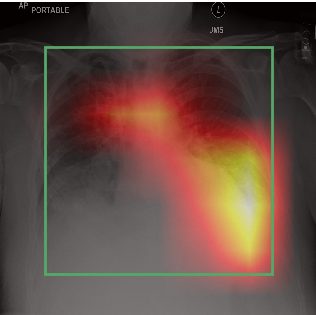
\includegraphics[width=0.3\textwidth]{images/preds/effusion_cam}\hspace{0.01\textwidth}%
  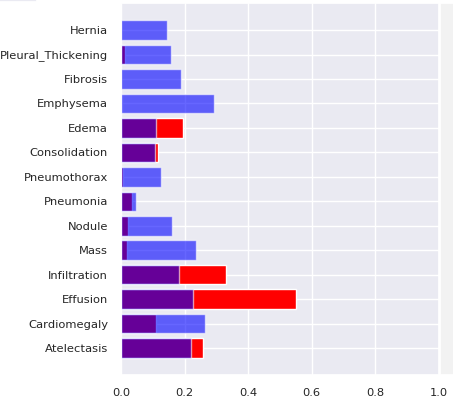
\includegraphics[width=0.3\textwidth]{images/preds/effusion_probs}\\[0.01\textwidth]
  \caption{Original image, image overlaid with saliency map and bounding boxes
    for \emph{Effusion}, and predicted probabilities for an x-ray image.}
  % \end{minipage}
  % }
  \label{examples_3}
\end{figure}
\end{frame}

\begin{frame}
\begin{figure}[H]
  % \fbox{
  % \begin{minipage}{\textwidth}
  \centering
  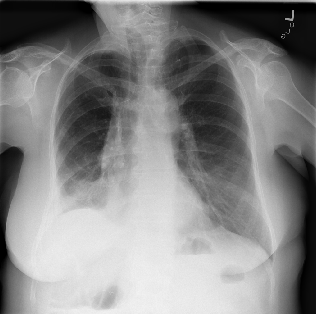
\includegraphics[width=0.3\textwidth]{images/preds/infiltration}\hspace{0.01\textwidth}%
  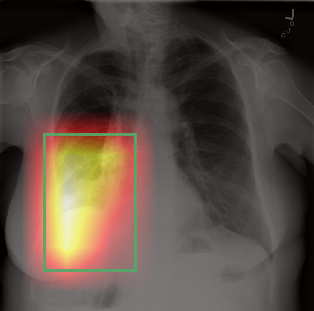
\includegraphics[width=0.3\textwidth]{images/preds/infiltration_cam}\hspace{0.01\textwidth}%
  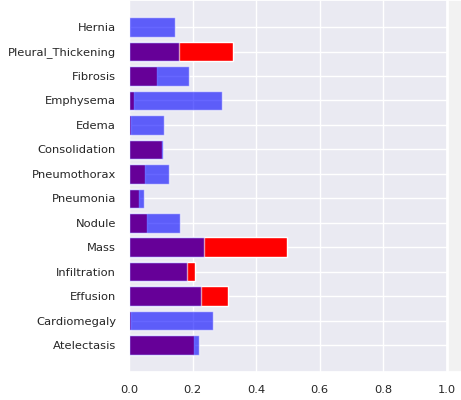
\includegraphics[width=0.3\textwidth]{images/preds/infiltration_probs}\\[0.01\textwidth]
  \caption{Original image, image overlaid with saliency map and bounding boxes
    for \emph{Infiltration}, and predicted probabilities for an x-ray image.}
  % \end{minipage}
  % }
  \label{examples_4}
\end{figure}
\end{frame}

\begin{frame}
\begin{figure}[H]
  % \fbox{
  % \begin{minipage}{\textwidth}
  \centering
  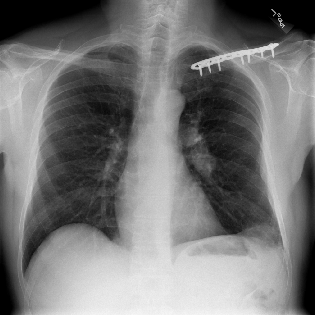
\includegraphics[width=0.3\textwidth]{images/preds/mass}\hspace{0.01\textwidth}%
  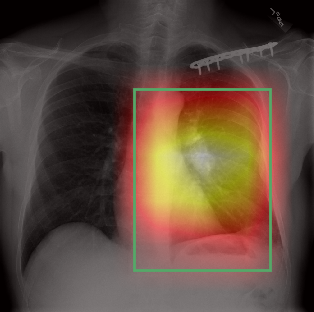
\includegraphics[width=0.3\textwidth]{images/preds/mass_cam}\hspace{0.01\textwidth}%
  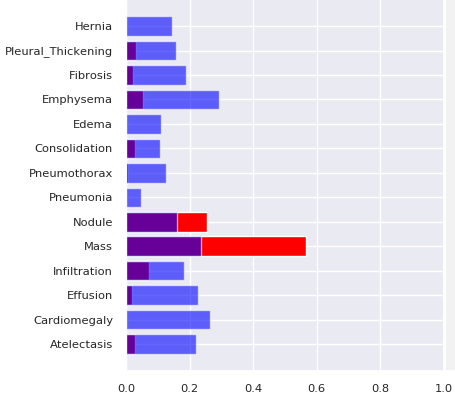
\includegraphics[width=0.3\textwidth]{images/preds/mass_probs}\\[0.01\textwidth]
  \caption{Original image, image overlaid with saliency map and bounding boxes
    for \emph{Mass}, and predicted probabilities for an x-ray image.}
  % \end{minipage}
  % }
  \label{examples_5}
\end{figure}
\end{frame}

\begin{frame}
\begin{figure}[H]
  % \fbox{
  % \begin{minipage}{\textwidth}
  \centering
  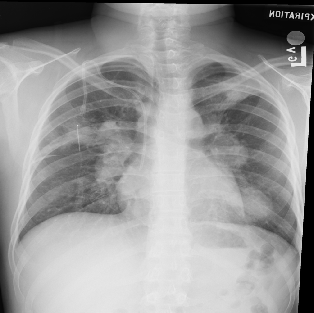
\includegraphics[width=0.3\textwidth]{images/preds/nodule}\hspace{0.01\textwidth}%
  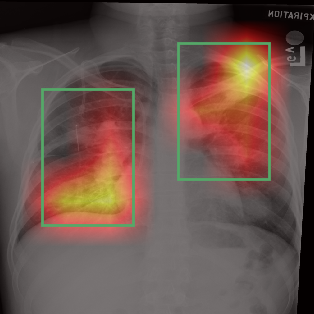
\includegraphics[width=0.3\textwidth]{images/preds/nodule_cam}\hspace{0.01\textwidth}%
  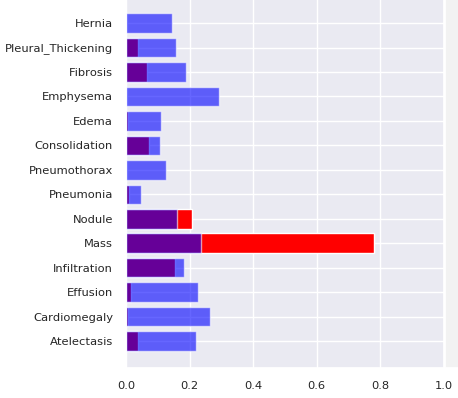
\includegraphics[width=0.3\textwidth]{images/preds/nodule_probs}\\[0.01\textwidth]
  \caption{Original image, image overlaid with saliency map and bounding boxes
    for \emph{Nodule}, and predicted probabilities for an x-ray image.}
  % \end{minipage}
  % }
  \label{examples_6}
\end{figure}
\end{frame}

\begin{frame}
\begin{figure}[H]
  % \fbox{
  % \begin{minipage}{\textwidth}
  \centering
  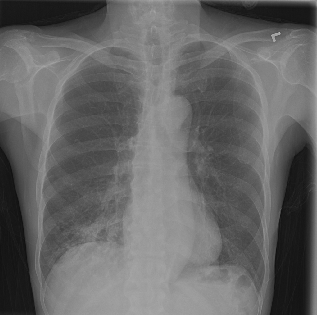
\includegraphics[width=0.3\textwidth]{images/preds/pneumonia}\hspace{0.01\textwidth}%
  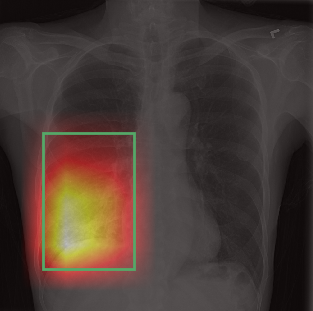
\includegraphics[width=0.3\textwidth]{images/preds/pneumonia_cam}\hspace{0.01\textwidth}%
  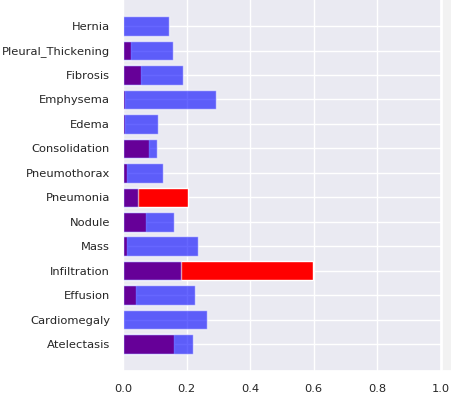
\includegraphics[width=0.3\textwidth]{images/preds/pneumonia_probs}\\[0.01\textwidth]
  \caption{Original image, image overlaid with saliency map and bounding boxes
    for \emph{Pneumonia}, and predicted probabilities for an x-ray image.}
  % \end{minipage}
  % }
  \label{examples_7}
\end{figure}
\end{frame}

\begin{frame}
\begin{figure}[H]
  % \fbox{
  % \begin{minipage}{\textwidth}
  \centering
  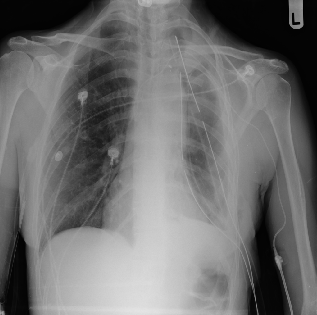
\includegraphics[width=0.3\textwidth]{images/preds/pneumothorax}\hspace{0.01\textwidth}%
  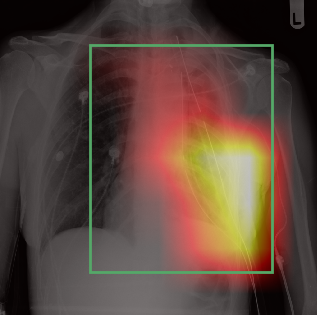
\includegraphics[width=0.3\textwidth]{images/preds/pneumothorax_cam}\hspace{0.01\textwidth}%
  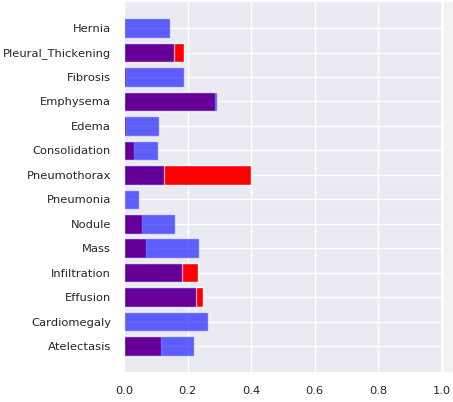
\includegraphics[width=0.3\textwidth]{images/preds/pneumothorax_probs}\\[0.01\textwidth]
  \caption{Original image, image overlaid with saliency map and bounding boxes
    for \emph{Pneumothorax}, and predicted probabilities for an x-ray image.}
  % \end{minipage}
  % }
  \label{examples_8}
\end{figure}
\end{frame}

\begin{frame}
\begin{figure}[H]
  % \fbox{
  % \begin{minipage}{\textwidth}
  \centering
  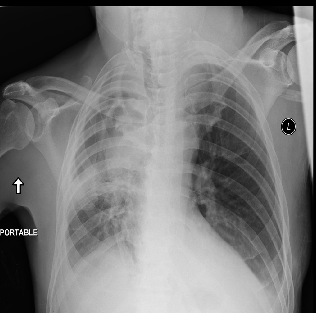
\includegraphics[width=0.3\textwidth]{images/preds/consolidation}\hspace{0.01\textwidth}%
  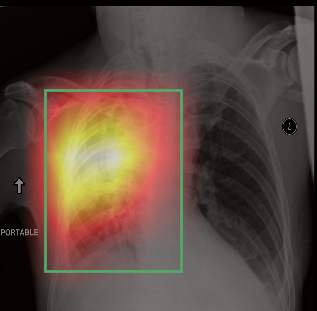
\includegraphics[width=0.3\textwidth]{images/preds/consolidation_cam}\hspace{0.01\textwidth}%
  \includegraphics[width=0.3\textwidth]{images/preds/consolidation_probs}\\[0.01\textwidth]
  \caption{Original image, image overlaid with saliency map and bounding boxes
    for \emph{Consolidation}, and predicted probabilities for an x-ray image.}
  % \end{minipage}
  % }
  \label{examples_9}
\end{figure}
\end{frame}

\begin{frame}
\begin{figure}[H]
  % \fbox{
  % \begin{minipage}{\textwidth}
  \centering
  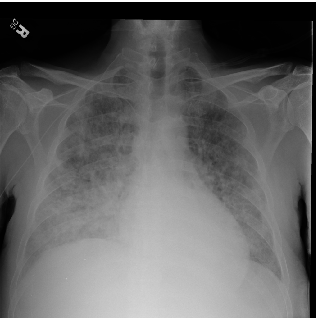
\includegraphics[width=0.3\textwidth]{images/preds/edema}\hspace{0.01\textwidth}%
  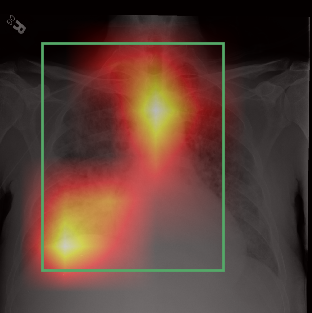
\includegraphics[width=0.3\textwidth]{images/preds/edema_cam}\hspace{0.01\textwidth}%
  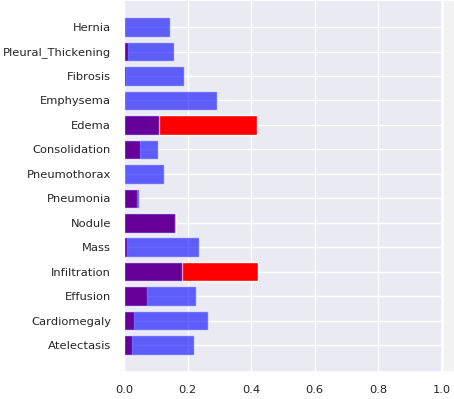
\includegraphics[width=0.3\textwidth]{images/preds/edema_probs}\\[0.01\textwidth]
  \caption{Original image, image overlaid with saliency map and bounding boxes
    for \emph{Edema}, and predicted probabilities for an x-ray image.}
  % \end{minipage}
  % }
  \label{examples_10}
\end{figure}
\end{frame}

\begin{frame}
\begin{figure}[H]
  % \fbox{
  % \begin{minipage}{\textwidth}
  \centering
  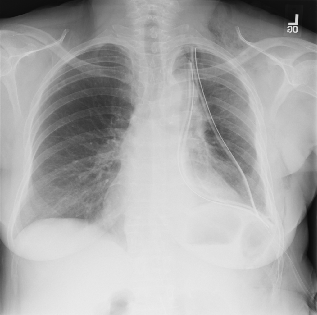
\includegraphics[width=0.3\textwidth]{images/preds/emphysema}\hspace{0.01\textwidth}%
  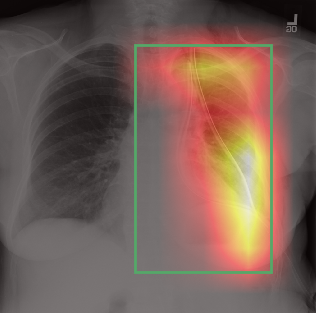
\includegraphics[width=0.3\textwidth]{images/preds/emphysema_cam}\hspace{0.01\textwidth}%
  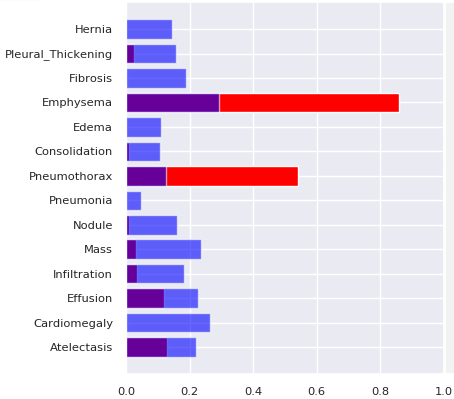
\includegraphics[width=0.3\textwidth]{images/preds/emphysema_probs}\\[0.01\textwidth]
  \caption{Original image, image overlaid with saliency map and bounding boxes
    for \emph{Emphysema}, and predicted probabilities for an x-ray image.}
  % \end{minipage}
  % }
  \label{examples_11}
\end{figure}
\end{frame}

\begin{frame}
\begin{figure}[H]
  % \fbox{
  % \begin{minipage}{\textwidth}
  \centering
  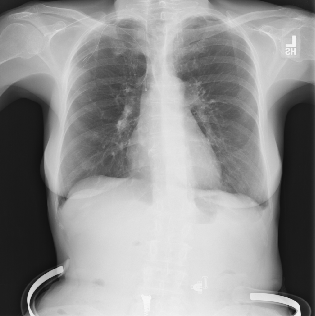
\includegraphics[width=0.3\textwidth]{images/preds/fibrosis}\hspace{0.01\textwidth}%
  \includegraphics[width=0.3\textwidth]{images/preds/fibrosis_cam}\hspace{0.01\textwidth}%
  \includegraphics[width=0.3\textwidth]{images/preds/fibrosis_probs}\\[0.01\textwidth]
  \caption{Original image, image overlaid with saliency map and bounding boxes
    for \emph{Fibrosis}, and predicted probabilities for an x-ray image.}
  % \end{minipage}
  % }
  \label{examples_12}
\end{figure}
\end{frame}

\begin{frame}
\begin{figure}[H]
  % \fbox{
  % \begin{minipage}{\textwidth}
  \centering
  \includegraphics[width=0.3\textwidth]{images/preds/PT}\hspace{0.01\textwidth}%
  \includegraphics[width=0.3\textwidth]{images/preds/PT_cam}\hspace{0.01\textwidth}%
  \includegraphics[width=0.3\textwidth]{images/preds/PT_probs}\\[0.01\textwidth]
  \caption{Original image, image overlaid with saliency map and bounding boxes
    for \emph{Pleural Thickening}, and predicted probabilities for an x-ray
    image.}
  % \end{minipage}
  % }
  \label{examples_13}
\end{figure}
\end{frame}

\begin{frame}
\begin{figure}[H]
  % \fbox{
  % \begin{minipage}{\textwidth}
  \centering
  \includegraphics[width=0.3\textwidth]{images/preds/hernia}\hspace{0.01\textwidth}%
  \includegraphics[width=0.3\textwidth]{images/preds/hernia_cam}\hspace{0.01\textwidth}%
  \includegraphics[width=0.3\textwidth]{images/preds/hernia_probs}\\[0.01\textwidth]
  \caption{Original image, image overlaid with saliency map and bounding boxes
    for \emph{Hernia}, and predicted probabilities for an x-ray image.}
  % \end{minipage}
  % }
  \label{examples_14}
\end{figure}
\end{frame}

\begin{frame}
\begin{figure}[H]
  % \fbox{
  % \begin{minipage}{\textwidth}
  \centering
  \includegraphics[width=0.3\textwidth]{images/preds/no_finding}\hspace{0.01\textwidth}%
  \includegraphics[width=0.3\textwidth]{images/preds/no_finding_cam}\hspace{0.01\textwidth}%
  \includegraphics[width=0.3\textwidth]{images/preds/no_finding_probs}\\[0.01\textwidth]
  \caption{Original image, image overlaid with saliency map and bounding boxes,
    and predicted probabilities for an x-ray image showing no abnormalities.}
  % \end{minipage}
  % }
  \label{examples_15}
\end{figure}
\end{frame}

\begin{frame}
\begin{figure}[H]
  % \fbox{
  % \begin{minipage}{\textwidth}
  \centering
  \includegraphics[width=0.45\textwidth]{images/preds/TB}\hspace{0.01\textwidth}%
  \includegraphics[width=0.45\textwidth]{images/preds/TB_cam}\\[0.01\textwidth]
  \caption{Original image, image overlaid with saliency map and bounding boxes
    for \emph{Tuberculosis}}
  % \end{minipage}
  % }
  \label{examples_16}
\end{figure}
\end{frame}

\begin{frame}
\begin{figure}[H]
  % \fbox{
  % \begin{minipage}{\textwidth}
  \centering
  \includegraphics[width=0.45\textwidth]{images/preds/TB2}\hspace{0.01\textwidth}%
  \includegraphics[width=0.45\textwidth]{images/preds/TB2_cam}\\[0.01\textwidth]
  \caption{Original image, image overlaid with saliency map and bounding boxes
    for \emph{Tuberculosis}}
  % \end{minipage}
  % }
  \label{examples_17}
\end{figure}
\end{frame}

\begin{frame}
  \frametitle{Prototype GUI}

  \begin{figure}[H]
    % \fbox{
    % \begin{minipage}{\textwidth}
    \centering \includegraphics[height=0.7\textheight]{images/pneumonia}
    \caption{A simple graphical user interface we created to let radiologists
      qualitatively evaluate predictions.}
    % \end{minipage}
    % }
    \label{screenshot}
  \end{figure}
  \end{frame}

\begin{frame}
  \frametitle{Future enhancements}

  \begin{enumerate}
  \item{Training on images from multiple hospital systems to improve the model's
      ability to generalize to other hospital systems and machine types, perhaps
      using techiniques in domain adaptation or deep domain confusion
      \cite{tzeng2014deep} to prevent the model from learning features that are
      necessary to identify the hospital system. }\pause
  \item{Exploring ways to infuse domain knowledge into the algorithm to exploit
      correlations between the abnormalities.}\pause
  \item{Using attention to allow the network to focus on pathological
      areas.}\pause
  \item{Training models end-to-end to generate radiology reports in natural
      language from x-ray images.}\pause
  \item{Segmentation of lung regions and bone shadow suppression to reduce the
      number of false-positives.}\pause
  \item{Using recently released datasets such as CheXPert\cite{Irvin2019} and
      PadChest\cite{Bustos2019} which have more images and a hierarchical
      labeling schema.}\pause
  \end{enumerate}

\section{References}
  
  \end{frame}
  \begin{frame}[allowframebreaks]
    \frametitle{References}
    \printbibliography
  \end{frame}
\end{document}


    